

\begin{figure}[t]
    \centering
    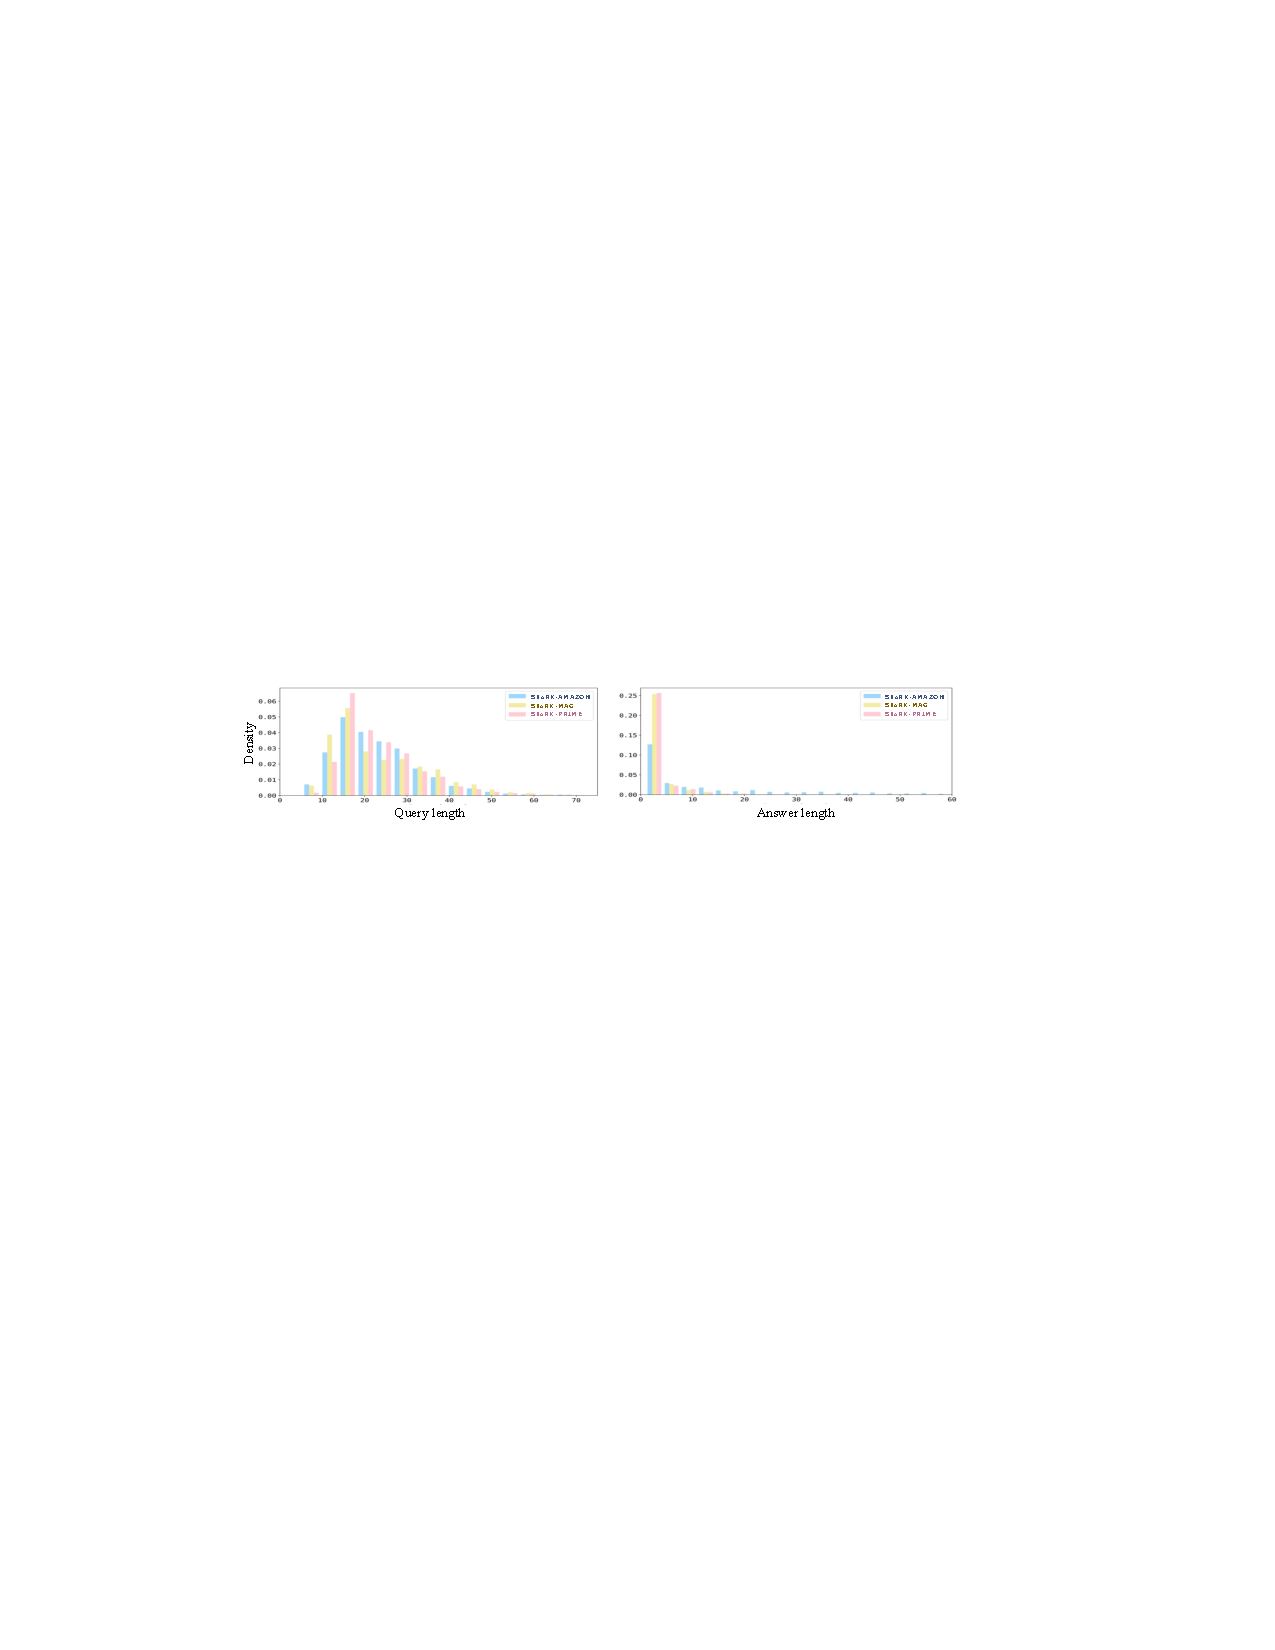
\includegraphics[width=1\textwidth]{figs/length_histv2}
    \vspace{-15pt}
    \caption{Distribution of query and answer lengths on \benchmarkh datasets.}
    \vspace{-5pt}
    \label{fig:length_dist}
\end{figure}

\begin{figure}[t]
    \begin{minipage}[t]{0.5\textwidth}
        \centering
      \captionof{table}{Query diversity measurement on \benchmarkt. \revision{See Appendix~\ref{app:math} for the metric definition.}}
      \vspace{5pt}
        \resizebox{1\textwidth}{!}{
        \begin{tabular}{l|cc}
            \toprule
            & {\small Shannon Entropy} & {\small Type-Token Ratio} \\
            % & {\small Entropy} & {\small Ratio} \\
            \midrule
            \small \amazonh & 10.39 & 0.179 \\
            \small \magh & 10.25 & 0.180 \\
            \small \primekgh & 9.63 & 0.143 \\
            \midrule
            \small Reference article & 10.44 & 0.261\\
            \bottomrule
        \end{tabular}
        }
        \label{tab:q_diversity}
    \end{minipage}%
    \hfill 
    \begin{minipage}[t]{0.47\textwidth}
        \caption{Average relative composition of relational vs. textual information.}
        \vspace{-5pt}
        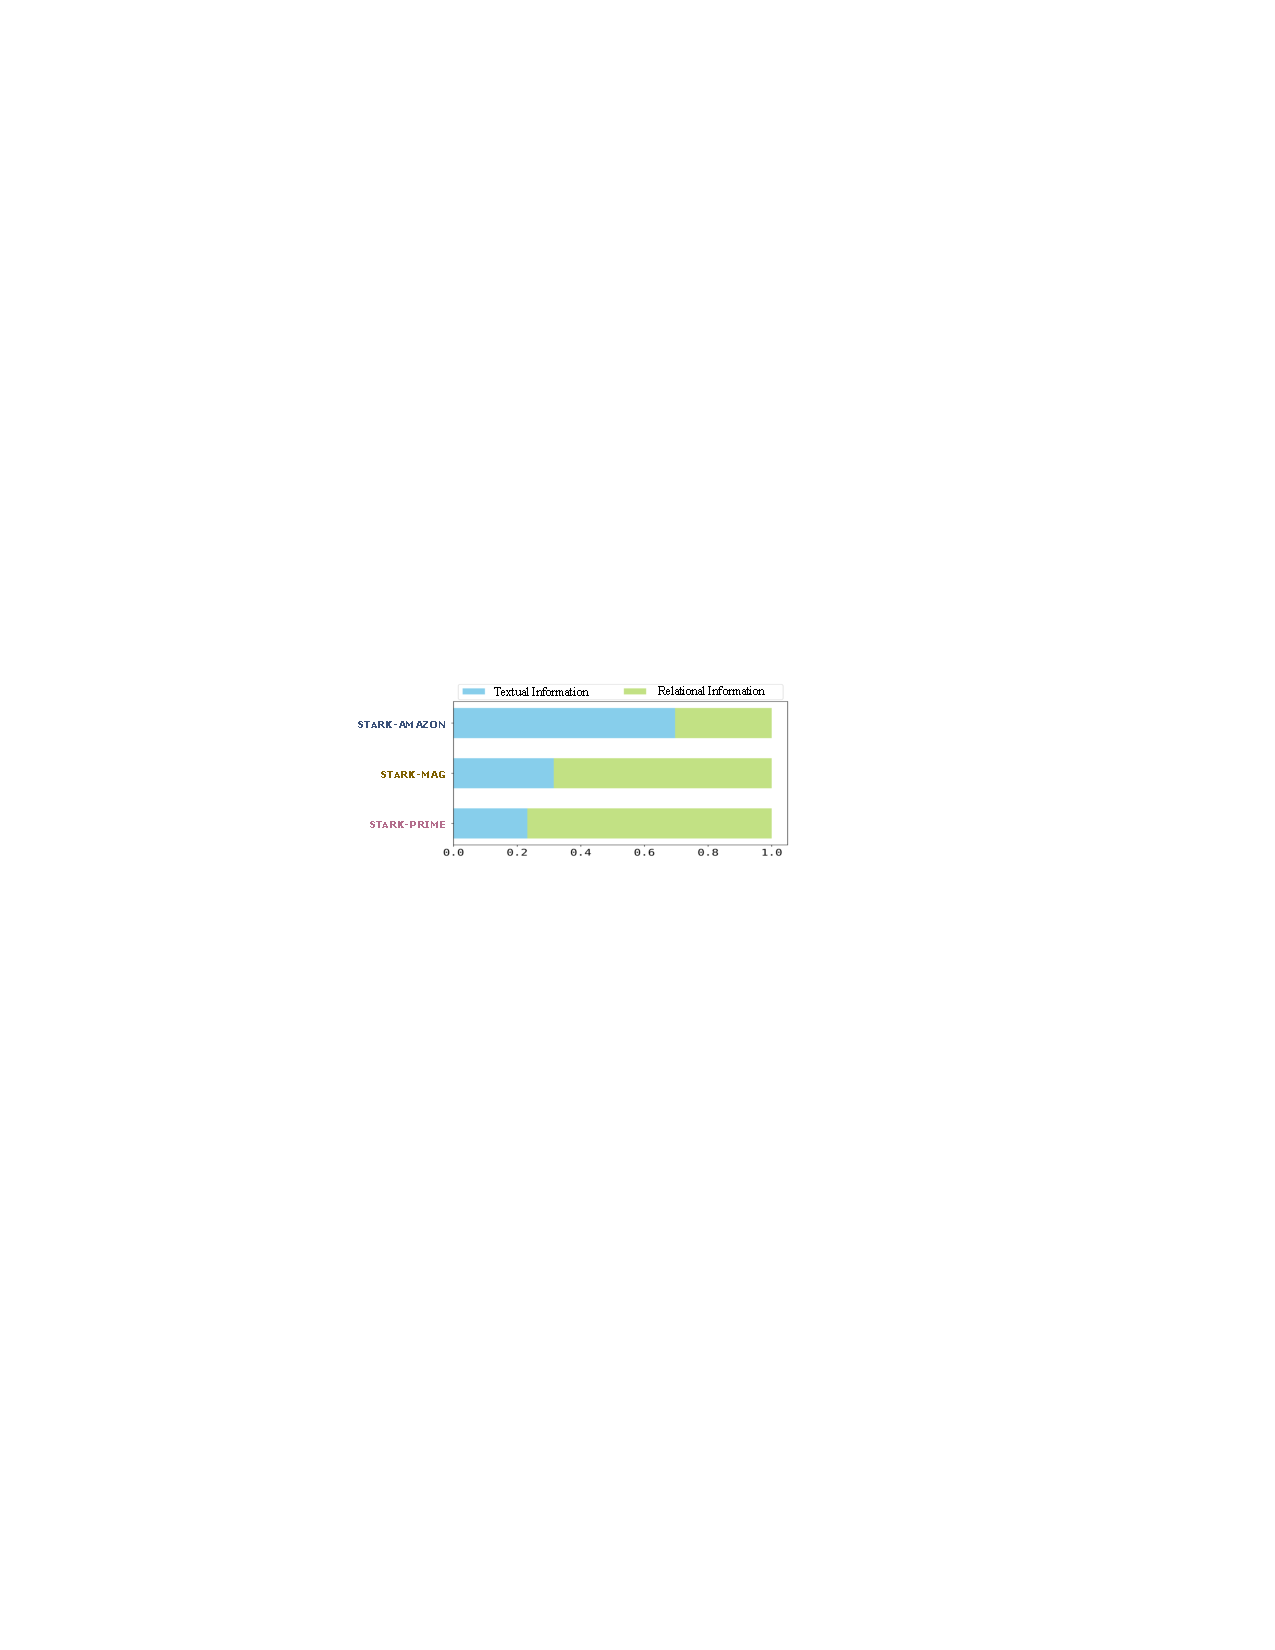
\includegraphics[width=\textwidth]{figs/ratiov2}
        \label{fig:ratio}
    \end{minipage}
    \vspace{-20pt}
\end{figure}


\subsection{Synthesized Data Distribution Analysis and Human Evaluation}
\label{sec:analysis}


% We conduct analysis and human evaluation on our synthesized datasets across three dimensions.
% to understand their characteristics and assess benchmark quality through human evaluation.
\begin{itemize}[leftmargin=*]
    \item \xhdr{Query and Answer Length} 
    Query length (in words) reflects the amount of user-provided context information, while the number of answers indicates query ambiguity/concreteness.
    Figure~\ref{fig:length_dist} shows similar query length distributions across the datasets, with most queries around 16 words. Longer queries (up to 50 words) often mention other entities or provide detailed context. Notably, 
    \amazonh has a significant long-tail pattern, with about 22\% of the answers have more than 30 entities, reflecting diverse e-commerce recommendations and ambiguous user queries.
    % , which results in a higher average answer length in 
    % Table~\ref{tab:benchmark_stats}
     
    \item \xhdr{Query Diversity} %  and Answer Coverage
    A diverse set of queries poses challenges for broader applicability to meet varying user demands. We measure query diversity using Shannon Entropy for word distribution and Type-Token Ratio (TTR) for unique words. Higher values indicate greater lexical diversity. Table~\ref{tab:q_diversity} shows high Shannon Entropy and steady TTR across all datasets. For reference, we compute these metrics for the Wikipedia page of Barack Obama\footnote{\url{https://en.wikipedia.org/wiki/Barack\_Obama}}. 
    
    \item \xhdr{Proportionality of Relational \textit{vs.}Textual Information}
    Our benchmark queries feature the composition of textual and relational information. To understand the distribution of information types, we calculate the average ratio of relational to textual requirements by word count in the queries across each dataset.  
    Note that the ratios do not directly reflect their importance in determining final answers. Figure~\ref{fig:ratio} shows varying ratios, which highlights different emphases on textual versus relational requirements and challenges retrieval systems to adapt to different distributions.

\end{itemize}

\xhdr{Human evaluation} 
We qualitatively assess sampled queries from our benchmark for naturalness (resembling natural conversation), diversity (covering various question structures and complexities), and practicality (relevance to real-world situations) with 63 participants. Evaluation results, converted from a 5-point Likert-like scale to a positive/tie/negative scale, show positive and non-negative rates in Table~\ref{tab:human} (Appendix~\ref{app:exp}). On average, 94.1\%, 85.3\%, and 89.4\% of participants rated the queries neutral or above in naturalness, diversity, and practicality, respectively. These results validate the quality of our benchmark and its potential for diverse and realistic retrieval tasks.
